\documentclass[../main.tex]{subfiles}

Fahren wir mit einem Sensor entlang der transmittierten Wellen nach der Beugung am Gitter, erwarten wir mittig vor dem Lötkolben ein starkes Signal, da hier das 0. Maximum des Interferenzmusters ist, wo die Wellen ohne Gangunterschied konstruktiv miteinander interferieren. Davor und dahinter sollten die 1. Maxima zu sehen sein, welche wir nicht so stark ausgeprägt erwarten, da hier ein Gangunterschied herrscht. Zwischen diesen Maxima sind logischerweise Minima zu erwarten, welche durch die destruktive Interferenz der IR-Wellen entstehen. Zu erwarten ist also ein Spektrum, welches diesem ähnelt (Abb. \ref{fig:ergebnisse-erwartetes-signal}):

\begin{figure}[ht]
    \centering
    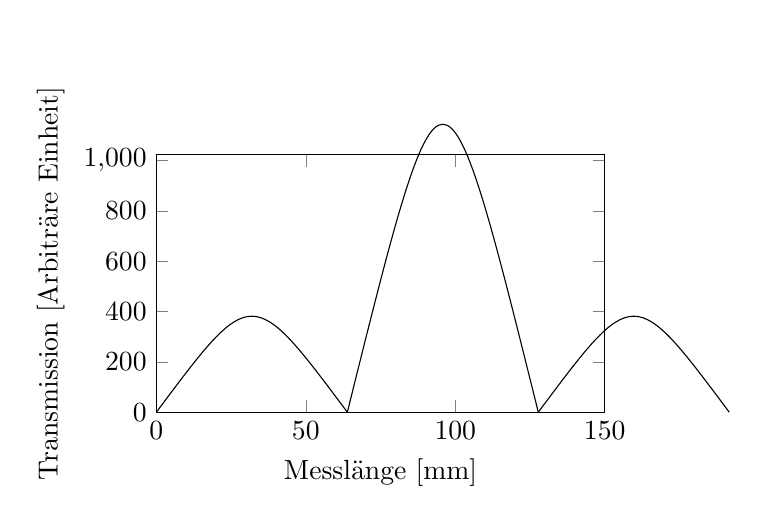
\begin{tikzpicture}
        \begin{axis}[
            xlabel={Messlänge [mm]},
            ylabel={Transmission [Arbiträre Einheit]},
            xmin=0, xmax=150,
            ymin=0, ymax=1023,
            width=0.6\textwidth,
            height=0.4\textwidth
        ]
        \end{axis}
        \begin{scope}[x={230},y={185}]
            \draw (0,0) .. controls (0.15,0.25) .. (0.3,0);
            \draw (0.3,0) .. controls (0.45,0.75) .. (0.6,0);
            \draw (0.6,0) .. controls (0.75,0.25) .. (0.9,0);
        \end{scope}
    \end{tikzpicture}
    \caption{Erwartetes Signal}
    \label{fig:ergebnisse-erwartetes-signal}
\end{figure}

\begin{figure}[ht]
    \centering
    \includegraphics[width=0.6\textwidth]{experiment/spectra/21c-diagramm-600-pro-mm.png}
    \caption{Signal des Lasers beim Durchfahren am Gitter (600 Linien pro mm)}
\end{figure}

% Fehler
